\section{Slope field}
\noindent\rule[\linienAbstand]{\linewidth}{\linienDickeDick}
Slope fields are often loead to a good qualitative understanding of the situation described by the ODE under consideration.
Slope field can be understood in the following way: To each point $(x, y)$ in the region $B$ under consideration, $F(x, y)$ is a value which discribes the slope of the solution curve passing through the point $(x, y)$.\\

\textbf{Example with calculator}\\
We want to plot the slope field of the following ODE
\begin{equation}
  y' = x - y
\end{equation}
\begin{table}[H]
  \setlength{\tabcolsep}{0.2em}
  \footnotesize
  \begin{tabular}{p{\linewidth / 2 - 0.5em}@{\hskip 1em}p{\linewidth / 2 - 0.5em}}
    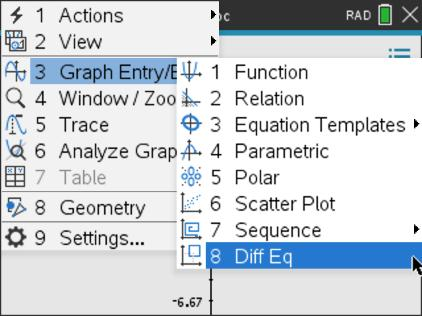
\includegraphics[width=\linewidth]{Pics/1.5.1.jpg} & 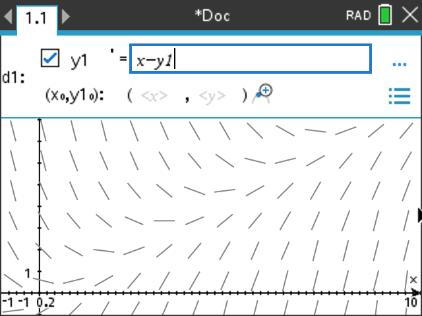
\includegraphics[width=\linewidth]{Pics/1.5.2.jpg} \\
    1. Select: Menu, 3: Graph Entry/Edit, 8: Diff Eq. & 2. Write down the ODE
  \end{tabular}
\end{table}
